\documentclass[11pt]{article}
\usepackage[margin=1in]{geometry}
\usepackage[T1]{fontenc}
\usepackage{graphicx}
\usepackage{booktabs}
\usepackage{caption}
\usepackage{titlesec}
\usepackage[hidelinks]{hyperref}

\captionsetup{font=small,labelfont=bf}
\titleformat{\section}{\normalfont\large\bfseries}{\thesection}{0.6em}{}
\titleformat{\subsection}{\normalfont\normalsize\bfseries}{\thesubsection}{0.5em}{}
\setlength{\parskip}{0.35em}
\setlength{\parindent}{0pt}

\title{\textbf{NeuroSense: Leakage-Aware, Explainable EEG Decoding}\\[0.3em]
\large An honest look at when EEG machine learning generalizes, and when it only appears to}
\author{Muizza}
\date{}

\begin{document}
\maketitle

\begin{abstract}
\noindent Machine learning on EEG is easy to evaluate incorrectly. Because EEG is a time series with strong short-range correlation, randomly splitting a single continuous recording into training and test sets lets a model score highly by recognizing near-duplicate neighbors rather than by learning a generalizable mapping. This report studies that failure across two datasets and two paradigms, under a single prespecified model and an evaluation protocol whose unit of inference is the subject rather than the epoch. On the widely used UCI EEG Eye State dataset, a naive random split gives a balanced accuracy of 0.533, while a chronological holdout falls to 0.416, below chance and far below the 0.767 majority baseline. On the PhysioNet Motor Movement/Imagery dataset, within-subject decoding of imagined left versus right fist reaches a mean per-subject AUC of 0.624 (95\% CI 0.536 to 0.721) with 8 of 10 subjects above chance, while cross-subject transfer sits at chance (balanced accuracy 0.482, CI 0.429 to 0.539). Feature attribution recovers the expected C3/C4 sensorimotor lateralization in Phase 2. In Phase 1 it recovers nothing interpretable, because the model it describes performs below chance; an earlier version of this work read those attributions as evidence of ocular artifact, and that reading is withdrawn here. Across both datasets, evaluation design determines apparent performance, and an explanation inherits the credibility of the evaluation beneath it.
\end{abstract}

\section{Introduction}
EEG underpins brain-computer interfaces, attention and fatigue monitoring, and a broad range of neurotechnology. Applying machine learning to EEG, however, requires care that is often skipped in introductory work: the signal is time-dependent, and samples that are close in time are highly correlated. When such samples are split randomly into training and test sets, a model can appear highly accurate while mostly recognizing repeated temporal patterns it has already seen, rather than learning structure that transfers to new data.

This report treats that pitfall as the object of study rather than an afterthought. It asks two questions. First, do the high accuracies commonly reported on a popular EEG benchmark survive leakage-aware evaluation? Second, on a dataset built for generalization, how far does honest decoding actually go, and do the model's explanations agree with known neurophysiology? The work is deliberately framed around evaluation validity and interpretability rather than headline accuracy, because on EEG a high number is only as trustworthy as the protocol that produced it.

A note on provenance. An earlier version of this report presented both phases with separate feature pipelines, different models per phase, and pooled epoch-level metrics. The analysis was subsequently rebuilt on a shared core with one band definition, preprocessing fitted inside each fold, and subject-level inference. Three claims from that earlier version did not survive the rebuild and are marked as withdrawn where they appear.

\section{Data and Methods}
\textbf{Phase 1: UCI EEG Eye State.} A single continuous 117-second recording from one subject, 14 channels sampled at 128\,Hz, labeled for eyes open versus closed. The label runs in only 24 contiguous blocks with a median duration of about 3.9 seconds, of which 19 contain at least one complete window. Several channels contain single-sample electrode pops reaching roughly 700{,}000 against a baseline near 4{,}000; these are clipped per channel, using thresholds fitted on training data only. The signal is segmented into one-second non-overlapping windows, yielding 100 windows and 56 band-power features. Every Phase 1 figure below therefore rests on 100 observations from a single person.

\textbf{Phase 2: PhysioNet Motor Movement/Imagery.} Imagined left versus right fist movement across 10 subjects at 160\,Hz, 437 trials in total drawn from runs R04, R08, and R12. Features are mu (8 to 13\,Hz) and beta (13 to 30\,Hz) band power over a 13-channel sensorimotor strip, giving 26 features per trial.

\textbf{Features.} For both phases, band power is computed per channel and window using Welch's method and integrated over each band. The delta, theta, alpha, and beta bands are used in Phase 1; the motor-relevant mu and beta bands in Phase 2. The lowest band edge is 1\,Hz rather than 0.5\,Hz, because a one-second Welch segment resolves frequency only to 1\,Hz. The gamma band (30 to 45\,Hz) is excluded, since on consumer-grade hardware that range is dominated by muscle activity rather than cortical signal.

\textbf{Model.} A single model is prespecified for both phases and all headline results: logistic regression with $C = 1.0$, balanced class weights, and a fixed random seed. Support vector machines and random forests appear only as secondary comparisons. Fixing one model in advance avoids the failure mode, present in an earlier version of this work, of assembling a headline result from the strongest metric of whichever model produced it.

\textbf{Evaluation.} All preprocessing, including artifact clipping, band-power extraction, and feature scaling, is fitted inside the cross-validation fold. For Phase 1 the grouping unit is the contiguous label block, since the dataset contains one subject; for Phase 2 it is the subject. In both cases one model is fitted per held-out group and that group's metrics are stored as a single row, so the headline figure is a mean over groups with a 95\% percentile bootstrap interval that resamples groups. Pooled epoch-level metrics are reported only as a descriptive appendix: pooling correlated epochs and treating them as independent both understates uncertainty and, for threshold-free metrics, distorts the estimate itself. A naive shuffled split is included in each phase purely as a contrast, to quantify the inflation that leakage produces.

\section{Results}

\begin{table}[h]
\centering
\small
\begin{tabular}{llccc}
\toprule
Phase & Protocol & Bal.\ accuracy & Macro F1 & ROC-AUC \\
\midrule
1 & Naive random window split & 0.533 & 0.533 & 0.566 \\
1 & Chronological 70/30 holdout & 0.416 & 0.330 & 0.491 \\
1 & Leave-one-block-out & 0.482 [0.334, 0.630] & 0.369 [0.239, 0.515] & undefined \\
\midrule
2 & Naive random trial split & 0.540 & --- & 0.525 \\
2 & Within-subject (trial CV) & 0.580 [0.493, 0.675] & 0.578 [0.490, 0.674] & 0.624 [0.536, 0.721] \\
2 & Cross-subject (LOSO) & 0.482 [0.429, 0.539] & 0.431 [0.380, 0.487] & 0.520 [0.439, 0.608] \\
\bottomrule
\end{tabular}
\caption{All results under the prespecified model. Brackets give 95\% percentile bootstrap intervals resampling blocks (Phase 1) or subjects (Phase 2). The majority baseline on the Phase 1 chronological test segment is 0.767.}
\label{tab:results}
\end{table}

\section{Phase 1: Eye-State Detection}
Because the label runs in long blocks, neighboring samples are near-identical and share a label. A random split scatters these neighbors across training and test, so a model scores well by recognizing duplicates. Holding everything else fixed and changing only how the split is drawn produces the performance gap shown in Figure~\ref{fig:leak}.

\begin{figure}[h]
\centering
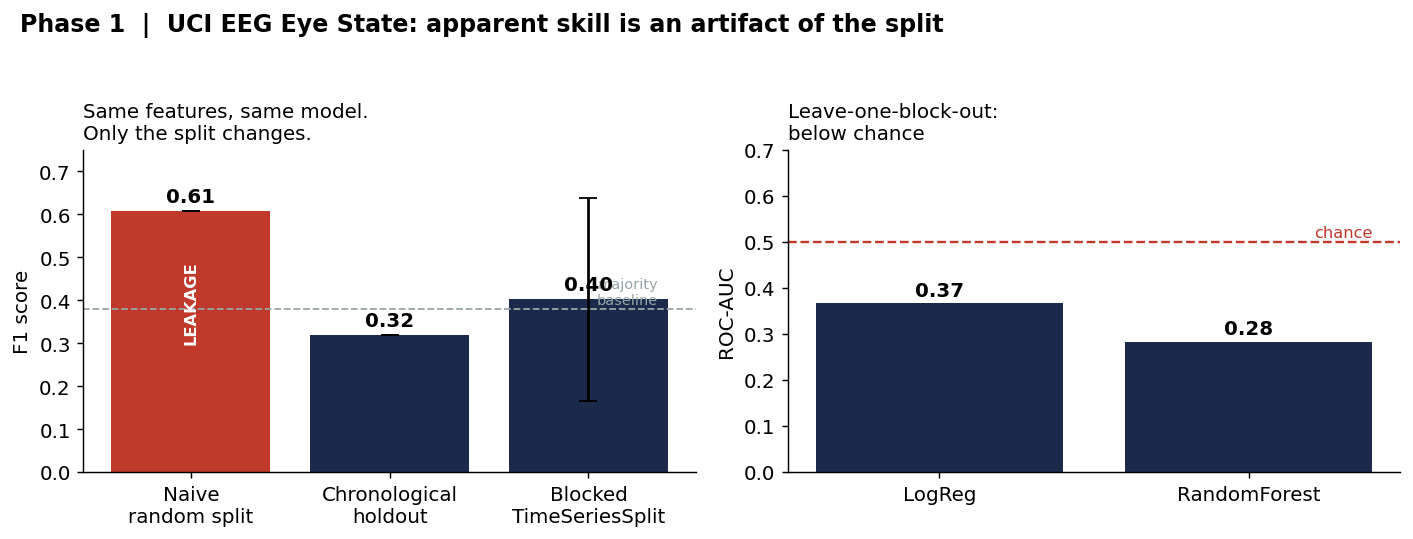
\includegraphics[width=\linewidth]{figures/fig1_phase1_leakage.png}
\caption{Left: balanced accuracy for the same features and model under three splits, with the chance level and the 0.767 majority baseline marked. Right: the per-block scores that the leave-one-block-out mean averages over, with its bootstrap interval shaded.}
\label{fig:leak}
\end{figure}

The leakage-aware protocols agree that nothing survives. The chronological holdout gives a balanced accuracy of 0.416, below chance, against a majority baseline of 0.767. Leave-one-block-out gives 0.482 with an interval of 0.334 to 0.630, an interval nearly half a unit wide because only 19 blocks and 100 windows are available.

One structural caveat deserves emphasis. Every contiguous label block is single-class by construction, so a held-out block contains only eyes-open or only eyes-closed windows. ROC-AUC cannot be computed on a single-class test set, and balanced accuracy degenerates into the recall of whichever class the block contains. An earlier version of this report gave a leave-one-block-out AUC range of 0.28 to 0.37 and read below-chance AUC as evidence that the features encode recording segment rather than eye state. That figure can only have come from pooling predictions across blocks, and the claim is withdrawn: the quantity it rests on is undefined at the level it was reported. Chronological holdout is the more interpretable leakage-safe protocol for this data, and leave-one-block-out is retained as a supporting check.

\subsection{Explainability, and its limits}
A pre-modeling check found no clean Berger effect in this recording: occipital alpha does not rise on eye closure. An earlier version went further and reported that the most class-separating features were frontal, reading this as ocular and blink artifact captured by frontal electrodes. That claim is withdrawn. Under the prespecified pipeline the top ten features are six frontal and four posterior or temporal, and the single strongest is temporal alpha at T7.

More fundamentally, the model these attributions describe scores 0.416 balanced accuracy, below chance. Permutation importance computed on a model that does not work is not evidence about physiology, and it is not evidence about artifact either. The honest conclusion is that Phase 1 yields no trustworthy explanation at all. That is itself the finding: an explanation inherits the credibility of the evaluation beneath it, and here there is none to inherit. What remains supported is the negative result, that a single continuous recording from one person cannot support generalizable eye-state decoding, and that accuracies reported on this dataset under random sample-level splits do not survive leakage-aware evaluation.

\section{Phase 2: Motor Imagery}
The same band-power approach is applied to data with many independent trials and multiple subjects. Two honest evaluations tell a two-part story (Figure~\ref{fig:gen}). Within a subject, trial-level cross-validation gives a mean per-subject balanced accuracy of 0.580 with an interval of 0.493 to 0.675, and a mean AUC of 0.624 with an interval of 0.536 to 0.721. The balanced-accuracy interval includes chance while the AUC interval excludes it, so the defensible claim is narrow: within-subject ranking is above chance, within-subject thresholded accuracy is not clearly so. Across subjects, leave-one-subject-out gives balanced accuracy 0.482 (0.429 to 0.539) and AUC 0.520 (0.439 to 0.608), both at chance. Individual subjects range from 0.365 to 0.637, a spread that a single pooled figure conceals entirely.

An earlier version reported cross-subject AUC as 0.48 and described it as below chance. That figure pooled every held-out subject's predicted probabilities into one array before scoring. Because subjects' decision scores sit on different scales, pooling manufactures apparent below-chance performance; the per-subject mean is 0.520. The conclusion is unchanged, chance either way, but the specific claim is withdrawn.

\begin{figure}[h]
\centering
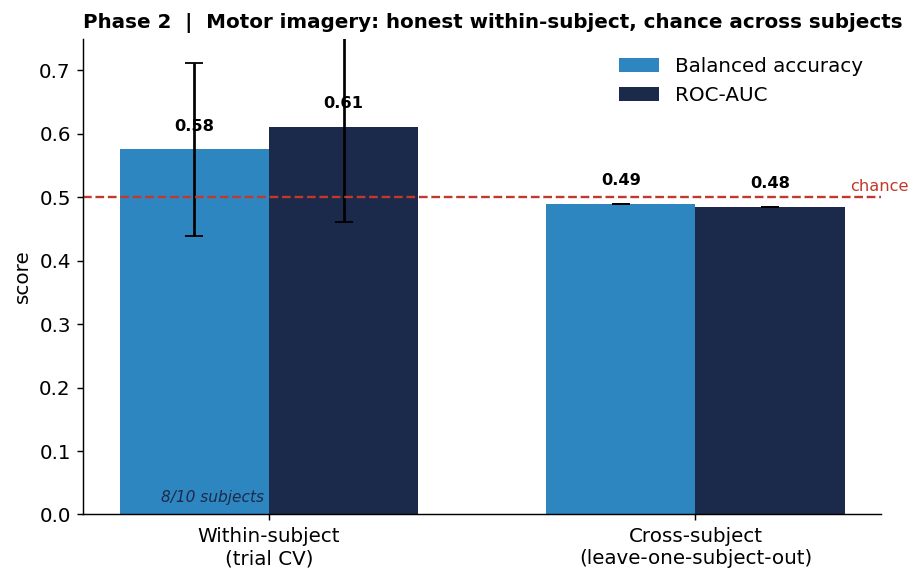
\includegraphics[width=0.72\linewidth]{figures/fig2_phase2_generalization.png}
\caption{Within-subject decoding is modestly above chance on AUC; cross-subject transfer sits at chance. Bars are subject means with 95\% bootstrap intervals; dots are the ten individual subjects.}
\label{fig:gen}
\end{figure}

The interpretability check here behaves very differently from Phase 1. The within-subject model keys on the C3 versus C4 mu rhythm (Figure~\ref{fig:interp}, right), the lateralized sensorimotor pattern expected from contralateral desynchronization during motor imagery. Here the attribution corroborates known physiology on a model that genuinely decodes.

\begin{figure}[h]
\centering
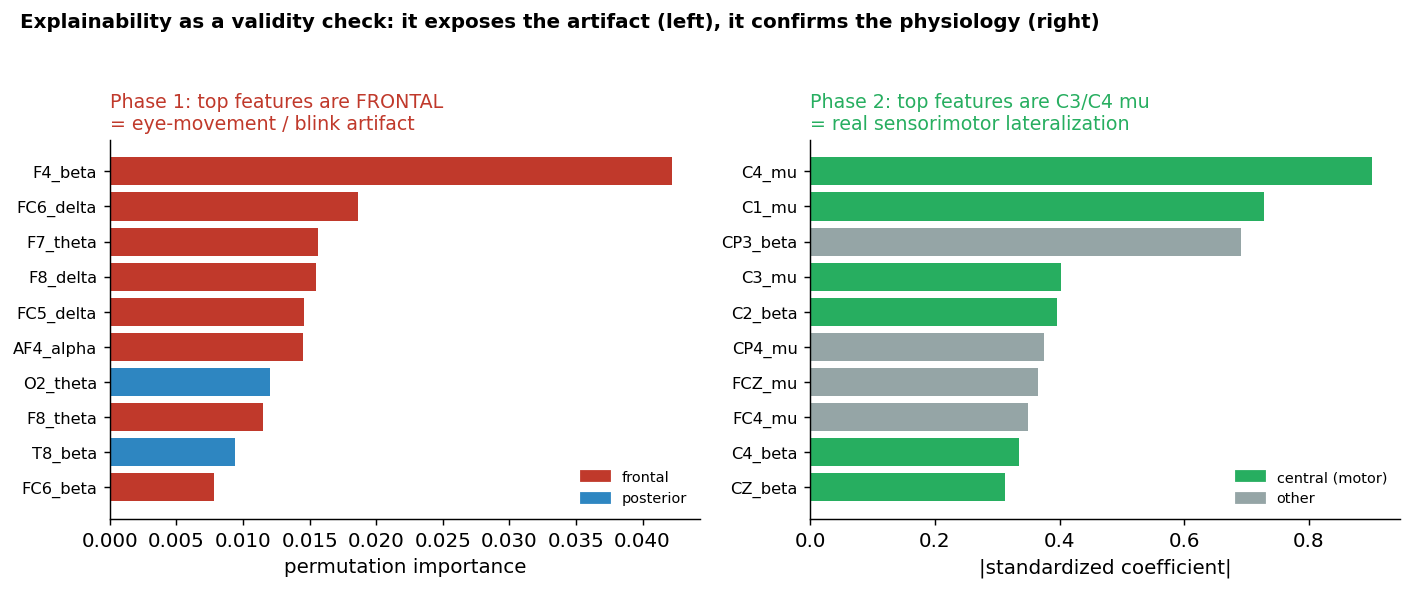
\includegraphics[width=\linewidth]{figures/fig3_interpretability_contrast.png}
\caption{Explainability is only as trustworthy as the evaluation beneath it. Right: Phase 2 top features sit on the central motor strip, consistent with sensorimotor lateralization, on a model that decodes above chance. Left: Phase 1 attributions on a model scoring 0.416, below chance, and therefore not readable as a finding in either direction.}
\label{fig:interp}
\end{figure}

\section{Discussion}
Across both datasets, naive evaluation overstates performance, and leakage-aware evaluation reveals that EEG band-power features capture structure other than the intended target: time and session structure in Phase 1, subject identity in Phase 2. Honest within-subject motor-imagery decoding is achievable but modest, and where it works its explanations align with sensorimotor physiology.

One caveat cuts against a tempting generalization. The naive random split inflates dramatically in Phase 1 but only mildly in Phase 2, where it reaches 0.540 against a cross-subject 0.482. Phase 2 uses discrete trials, and random splitting of discrete trials leaks far less than random splitting of continuous windows. How much a naive split inflates depends on how much temporal structure the epochs share, so the dramatic result belongs to Phase 1 and should not be stated as a general law of EEG machine learning.

Taken together, the two phases make a single point: model explanations are usable as evidence only when the evaluation beneath them is leakage-free. The corollary, learned the hard way in the course of this work, is that where the evaluation shows a model failing, its attributions should be reported as uninterpretable rather than mined for a plausible story. An attribution plot on a broken model is a confident description of nothing.

\section{Limitations}
Phase 1 is a single subject and single session recorded on consumer-grade hardware, so its results are not subject-generalizable and its high-frequency content is unreliable. Windowing produces only 100 windows, which is why every Phase 1 interval is wide, and its single-class label blocks make leave-one-block-out only partially interpretable. Phase 2 uses 10 of the 109 available subjects, so its intervals are wider than necessary. The two phases also differ in hardware, channel count, and sampling rate, so any comparison between them confounds paradigm with recording setup; the contrast between them is offered as a hypothesis rather than a controlled result.

\section{Future Work}
The natural next steps are to scale Phase 2 to all 109 subjects to tighten the estimates, to add common spatial pattern (CSP) features that are standard for motor imagery, and to attempt subject-adaptive transfer, both unsupervised alignment and small-sample calibration, to lift cross-subject decoding above chance. A third phase on mental arithmetic is planned, with its hypotheses, ablations, and primary endpoint fixed in advance in a committed preregistration. Deep models are deferred until these leakage-safe baselines are established.

\begin{thebibliography}{9}
\small
\bibitem{uci} R\"osler, O. and Suendermann, D. (2013). A First Step towards Eye State Prediction Using EEG. UCI Machine Learning Repository, dataset 264: EEG Eye State.
\bibitem{schalk} Schalk, G., McFarland, D. J., Hinterberger, T., Birbaumer, N., and Wolpaw, J. R. (2004). BCI2000: A General-Purpose Brain-Computer Interface System. \textit{IEEE Transactions on Biomedical Engineering}, 51(6), 1034--1043.
\bibitem{physionet} Goldberger, A. L. et al. (2000). PhysioBank, PhysioToolkit, and PhysioNet. \textit{Circulation}, 101(23), e215--e220. EEG Motor Movement/Imagery Database v1.0.0.
\bibitem{berger} Berger, H. (1929). Uber das Elektrenkephalogramm des Menschen. \textit{Archiv fur Psychiatrie und Nervenkrankheiten}, 87, 527--570.
\end{thebibliography}

\end{document}
